\documentclass{article}
\usepackage[utf8]{inputenc}
\usepackage{graphicx}
\usepackage{amsmath,amsthm,amssymb}
\usepackage{indentfirst}
\usepackage{bbold} %package to type identity matrix \mathbb{1}
\usepackage[colorlinks,linkcolor=blue,urlcolor=blue,citecolor=blue]{hyperref}
\usepackage[top=1in, bottom=1in, left=1in, right=1in]{geometry}
\usepackage{float}

\title{Summary for Low-rank matrix completion}
\author{Jingwen Liang}
\date{November 2014}

\begin{document}

\maketitle

\section{Introduction}
One needs roughly $rn$ parameters to specific an $n\times n$ matrix $A$ of rank $r$. Thus it can be implied that about same number of expansion coefficients of $\rho$ (use some fix matrix basis) are sufficiently to unique specify $\rho$ within the set of low-rank matrices. It is by far less clear whether $\rho$ can be recovered from this limited set of coefficients in a computationally tractable way. 

\subsection{3 main improvements were achieved:}
\begin{enumerate}
\item Most importantly, the mathematical effort for obtaining {\color{red}near-optimal bounds} on the number of coefficients needed to determine a Low-rank matrix was {\color{blue}cut dramatically}, with a {\color{blue}condensed (but complete) version of the proof} fitting on a single page.

\item the new arguments depend much less on the specific properties of the basis used.

\item In some situations, {\color{blue}the bounds obtained are tighter than those presented previously}. In some cases, the gap between lower and upper bounds is reduced to a multiplicative constant.


\end{enumerate}

\subsection{Question}
Given that rank $ (\rho) \le r $,
how many randomly chosen coefficients $(w_a,\rho)$ do we need to know, before we can efficiently reconstruct $\rho$?
\subsection{Algorithm}
convex optimization over the space of matrices:
\begin{equation}
\begin{aligned}
& {\text{min}}
& & \| \sigma \|_* \\
& \text{subject to}
& & ( w_a,\sigma) = (w_a, \rho) , \qquad \forall a \in \Omega.
\end{aligned}
\end{equation}







\subsection{Setting}
\begin{enumerate}
\item Matrices are``Hermitian Matrix"------$\sigma^* = \sigma$;

\item $\rho$ is the Unknow low-rank (with rank-$r$) matrix that we want to recover;

\item Inner product:
\begin{align*}
& (\sigma_1, \sigma_2) = tr(\sigma_1^*\sigma_2) 
& &  \text {The Hilbert-Schmidt inner prodect}\\
& <\psi,\phi>  = \psi^*\phi 
& & \text {The standard inner prodect in} \mathbb{C}^n;
\end{align*}


\item {\color{blue}Ortho-normal basis} $\{w_a\}^{n^2}_{a=1}$ with respect to this inner product has been chosen. Thus, $\rho$ can be expanded as $\rho = \sum_{a=1}^{n^2}(w_a,\rho) w_a$;

\item $\Omega\subset[1,n^2]$  be a random set of size $m$ which is roughly $O(rn)$ coordinates we have information about.
$\Omega^{\perp}$ is the set of coordinates that we have no information;

\item $\sigma^*$ is the solution of the optimization;

\item Consider $\rho = U S_r U^*$, where $S_r \in \mathbb{C}^{r \times r}$, is the diagonal matrix with singular values of $\rho$ on its diagonal. $U \in \mathbb{C}^{n\times r}$ whose colomns are orthogonal to each other if you extend $U$ to $V=[U|U^\perp]$ then V is unitary $n\times n$ matrix, i.e. $V^*V = VV^* = \mathbb{1}$ and the singular value decomposition gives us $\rho = V\Sigma V^*$;

\item Let $u_k$ denote the $k$th colomn of $U$, $U=\text{span}(u_1,\dots,u_r)= \text{range }\rho$ (row space and column space of $\rho$)


\item $P_U$ orthogonal projection onto $\text{range } \rho$. The range of $\rho$ can be achieve by apply $\rho$ to any vector $x \in \mathbb{C}^n$  Apply $P_U$ on vectors in range of $\rho$ makes no change since $P_U$ is orthogonal projection onto $\text{range } \rho$.

i.e. $\rho x \in \text{range } \rho$.

$P_U\rho x = P_UU\Sigma U^*x=U\Sigma U^*x = \rho x$ . Thus $P_U= UU^*$.

 
\item $T = \{ \sigma | (\mathbb{1} - P_U) \sigma(\mathbb{1} - P_U) = 0 \}$ is the space of matrices whose {\color{red} compression} to $ker \rho$ vanishes. 
\begin{align*}
\mathbb{1}-P_U &= \mathbb{1}-UU^* = VV^* - UU^*\\
&= \begin{bmatrix}
U & U^{\perp}
\end{bmatrix}\begin{bmatrix}
U^* \\U^{\perp^*}
\end{bmatrix}-UU^*\\
&=UU^*+U^\perp U^{\perp^*}-UU^*\\
&=U^\perp U^{\perp^*}\\
&=P_U^\perp
\end{align*}
Set T is set of matrix that is somehow ``orthogonal'' to $\rho$
.Think about what kind of $\sigma$ can I put in  $U^\perp
 U^{\perp^*}\sigma U^\perp U^{\perp^*}$ then get 0. It is any thing that is spanned by columns of U, because $U^\perp U = 0$. 
 
$T$ is the linear space spanned by elements of the form $u_k x^*$ and $xu_k^*$, $1 \le k \le r$ where $x$ is arbitrary
 
\item $T^\perp$ the orthogonal complements of $T$. $T^\perp$ is the subspace of matrices spanned by the family $xx^*$ where $x$ is any vector orthogonal to U.

\item Orthogonal decomposition $\mathbb{R}^{n\times n} = T \oplus T^\perp$ .

\item The orthogonal projection onto $T$ is given by
\[
\mathcal{P}_T(\sigma) = P_U \sigma + \sigma P_U - P_U \sigma P_U
\]
 ($\mathcal{P}_T$ for matrix valued projection and $P$ for vector valued projection)
 


\item The orthogonal projection onto $T^\perp$ is given by 
\[\mathcal{P}_{T^\perp}(\sigma)=(\mathbb{1}-\mathcal{P}_T)(\sigma)=(\mathbb{1}-P_U)\sigma(\mathbb{1}-P_U)
\]

\item decompose $\Delta = \Delta_T + \Delta_{T}^\perp$, with $\Delta_T \in T$, $\Delta_T^\perp \in T^\perp$.

\item $m = nr\kappa$. $\kappa$ is the "oversampling factor" which describes {\color{red}the leverage we allow ouerselves by going beyond the minimum number of parameters needed to describe $\rho$}

\item Let $s_i$ be singular value of a matrix $\sigma$. The usual matrix norm are 
\begin{equation}
\begin{aligned}
& \| \sigma \|_{op}
& & = \underset{i} {\mathrm{max}} ~s_i & &\text{ (Operator/spectral norm)}\\
& \| \sigma \|_*
& & = tr | \sigma | = \left(\sum_i s_i\right) & &\text{ (Trace norm)}\\ 
& \| \sigma \|_F
& & = (\sigma,\sigma)^{1/2} = \left(\sum_i s_i^2\right)^{1/2} & &\text{ (Frobenius norm)}.
\end{aligned}
\end{equation}

\item Both the identity matrix and the identity function on more general spaces are denoted by $\mathbb{1}$.

\item Inequality between matrix: $\sigma_1 \preceq \sigma_2$ i.f.f. $\sigma_1 - \sigma_2$ is positive semi-definite {\color{red}(a convention sometimes referred to as matrix order or L$\ddot{o}$wner partinal order)}.

\item sign function:

\textbf{For scalar:} $sgn(x) = x/|x|$ for $x \neq 0$ and $sgn(0) = 0$.

\textbf{For ``Hermitian matrix":} $\text{sgn }  (\sigma)$ is the diagonal matrix in the same basis as $\sigma$ but with eigenvalues $\text{sgn }(\lambda_i)$, where $\lambda_i$ are the eigenvalues of $\sigma$.

\item 
Let $A_1, \dots, A_m$ be $m$ random variables taking values in $[1,n^2]$.($A_1, \dots ,A_m \in \Omega \subset [1,n^2]$ )

The sampling operator
$\mathcal{R}: \sigma  \mapsto \dfrac{n^2}{m} \sum_{i=1}^m w_{A_i}(w_{A_i}, \sigma)$


\end{enumerate}




\section{incoherence}
\textbf{Definition 1} (Coherence).\textit{The $n \times n$-matrix $\rho$ has coherence $\nu$ with respect to an operator basis $\lbrace w_a\rbrace_{a=1}^{n^2}$ if either}
\[
\underset{a} {\mathrm{max}} ~\|w_a\|_{op}^2 \le \nu \dfrac{1}{n},
\]
or
\begin{align*}
\underset{a} {\mathrm{max}} ~\|\mathcal{P}_Tw_a\|_F^2 &\le 2\nu \dfrac{r}{n},\\
\underset{a} {\mathrm{max}} ~~(w_a,\text{sgn}\rho)^2 &\le \nu\dfrac{r}{n^2}
\end{align*}
\textit{hold.}
\\[1ex]

If $\rho$ has few non-zero expansion coefficients w.r.t. the basis $\{w_a\}$, the algorithm will perform bad. We need  incoherence to avoid such situation ------ must ensure that a typical coefficient will contain ``enough non-trivial information'' about $\rho$.
\subsection{matrix incoherence explanition}
The paper find that there are certain bases with the property that ANY low-rank matrix is incoherent w.r.t them.

{\color {blue}Matrices with small operatior norm (spectral norm) $\max_a \|w_a\|_{op}$ are ``incoherent" to all low-rank matrices simultaneously.}

Detial: If $\rho$ is a matrix of rank $r$, normalized such that $\| \rho \|_F = 1$, then H$\ddot{o}$lder's inequality for matrices gives the estimate 

\begin{equation}
|(w,\rho)|^2 \le \|w\|_{op}^2 \|\rho\|_*^2 \le \|w\|_{op}^2 r
\end{equation} 
for any matrix $w$. Hence the squared overlap on the left hand side is small if both $r$ and $\|w\|$ are. As a corollary, we can actually derive $\underset{a} {\mathrm{max}} ~\|\mathcal{P}_Tw_a\|_F^2 \le 2\nu \dfrac{r}{n}$ from $\underset{a} {\mathrm{max}} ~\|w_a\|_{op}^2 \le \nu \dfrac{1}{n}$. Indeed
\begin{align*}
\|\mathcal{P}_T w_a\|_F^2 & = \sup_{_{\sigma\in T,\|\sigma\|_F = 1}}(w_a,\sigma)^2 \\
& \le \|w_a\|_{op}^2\|\sigma\|_*^2\\
& \le \|w_a\|_{op}^2 2r\|\sigma\|_F^2\\
& \le 2\nu\dfrac{r}{n}
\end{align*}
since $\max_{_{\sigma\in T}}(\text{rank }\sigma) = 2r $. T is spanned by $U_kx^*$ and $xU^*$ which is at most the linear combination of $2r$ independent bases.


\section{Main Result}
\textbf{Theorem 3} \textit{Let $\rho$ be a rank-$r$ matrix with coherence $\nu$ with respect to an operator basis $\lbrace w_a \rbrace_{a=1}^{n^2}$. Let $\Omega \in [1,n^2]$ be a random set of size $|\Omega|=m \ge O(nr\nu^{(1+\beta)}\ln^2n)$. Then the solution $\sigma^*$ of the optimization problem (1) is unique and equal to $\rho$ with probability at least $1-n^{-\beta}$.}

\[
|\Omega|=m > \log_2(2n^2\sqrt{r}) 64\nu(\ln(4n^2)+\ln(9\log_2n)+\beta\ln n) rn
\]

\section{Intuition}
Known information: space spanned by the $\lbrace w_a | a \in \Omega\rbrace$. There is a large affine space of matrices compatible with the available information. Goal is to specify an algorithm which picks one point from the high-dimensional affine space, and prove that our choice is identical to $\rho$ with high probability. After used \textit{trace heuristic} instead of lowest-rank, the objective thus becomes proving that the trace-norm restricted to the affine plane has a strict and global minimum at $\rho$. 

If $\rho + \Delta \neq \rho$ is any matrix in the affine plane, we need to show that 
\begin{equation}
\|\rho + \Delta\|_* > \|\rho\|_*
\label{eq:4}
\end{equation}

\textbf{A short handwaving argument: }\textit{Adding a generic deviation $\Delta$ to a low-rank $\rho$ is indeed likely to increase the trace-norm.}
\begin{proof}
{\color{red}Recall that the trace norm of a matrix is larger that the sum of the absolute values of the elements on the main diagonal.} Let $\rho_1, \dots, \rho_r$ be the eigenvalues of $\rho$. Then

\begin{equation}
\begin{aligned}
\|\rho + \Delta\|_* \quad
&  \ge \quad \sum_{i=1}^r|\rho_i + \Delta_{i,i}| + \sum_{i = r+1}^n|\Delta_{i,i}|\\
&  \ge  \quad \|\rho\|_* + \sum_{i=1}^r (\text{sgn }\rho_i)\Delta_{i,i} + \sum_{i = r+1}^n |\Delta_{i,i}|
\end{aligned}
\label{eq:5}
\end{equation}
For \textit{generic} derivations $\Delta$, we expect that the $\Delta_{i,i}$ all have comparable magnitudes. Therefore, as long as $r\ll n$, the second sum in (\ref{eq:5}) will dominate the first one as required.
\end{proof}


The only {\color{blue}difficulty faced in this paper consists in proving that $\|\rho + \Delta\|_* > \|\rho\|_*$ holds not just for generic matrices $\rho + \Delta$ in the aforementioned affine plane, but for {\color{red}all such elements} simultaneously.} Key to that will be a simple concept from convex optimization theory:{ \color{red}\textit{a dual certificate}}. By that we mean a matrix $Y$ such that 
\begin{equation}
\|\rho + \Delta\|_* > \|\rho\|_* + (Y, \Delta)
\end{equation}

For $\Delta \neq 0$. If we can find such a $Y$ which is also normal to the affine space, then the inner prodect above vanishes and $\|\rho + \Delta\|_* > \|\rho\|_* + (Y, \Delta)$ implies $\|\rho + \Delta\|_* > \|\rho\|_*$.

\section{Main Proof}
\subsection{\textit{The ensemble}}
\begin{enumerate}
\item Let $A_1,\dots,A_m$ be random variables taking values in $[1,n^2]$ with distribution {\color{red}specified momentarily}.

\item $w_{A_i}$ ----- random matrices

\item sampling operator: 
\begin{equation}
\mathcal{R}: \sigma \mapsto \dfrac{n^2}{m}\sum_{i=1}^{m} w_{A_i}( w_{A_i},\sigma)
\label{eq:7}
\end{equation}

\item analyze the semi-definite program

\begin{equation}
\begin{aligned}
&\text{min} 
& &  \|\sigma\|_*\\
&\text{subject to} 
& & \mathcal{R}\sigma = \mathcal{R}\rho
\end{aligned}
\label{eq:8}
\end{equation}

\item \textbf{Two type of solutions} The solution $\sigma^*$ to 
\begin{equation}
\begin{aligned}
&\text{min} 
&    &  \|\sigma\|_*\\
&\text{subject to} 
&     &\mathcal{R}\sigma = \mathcal{R}\rho
\end{aligned}
\label{eq:9}
\end{equation}

is unique and equal to $\rho$ if and only if any non-zero deviation $\Delta = \sigma - \rho$ from $\rho$ is eigher \textit{infeasible}
\begin{equation}
\mathcal{R}\Delta \neq 0,
\label{eq:10}
\end{equation}
or causes the trace-norm to increase
\begin{equation}
\|\rho+\Delta\|_* > \|\rho\|_*
\label{eq:11}
\end{equation}


\item \textbf{Sample \textit{without} replacement:} If the $A_i$'s correspond to $m$ samples drawn frmo $[1,n^2]$ \textit{without} replacement, the programs
\begin{equation}
\begin{aligned}
& {\text{min}}
& & \| \sigma \|_* \\
& \text{subject to}
& & (\sigma, w_a) = (\rho, w_a) ,\qquad \forall a \in \Omega.
\end{aligned}
\end{equation}
and 
\begin{equation}
\begin{aligned}
&\text{min} 
&    &  \|\sigma\|_*\\
&\text{subject to} 
&     &\mathcal{R}\sigma = \mathcal{R}\rho
\end{aligned}
\end{equation}

are equivalent.

\item \textbf{Sample \textit{with} replacement; collisions:} Consider $A_i$'s are i.i.d. random variables. Due to independent, the situation is much easier to analze, but also imples the possibility of \textit{collisions}. In the presence of collision, fewer than $m$ distinct coefficients will contribute to (\ref{eq:8}). And thus plausible that any upper bound on the probability of failure of the i.i.d. scheme is also valid for \textit{no replacement} situation.

Thus, we can assume $A_i$'s are i.i.d random variables.

Using (\ref{eq:10})$\mathcal{R}\Delta \neq 0$, we can give a simple proof of our earlier remark that sampleing with replacement can only decrease that probability of recovering $\rho$:
\end{enumerate}

\begin{proof}
Let $p_{with}(m)$, $p_{wout}(m)$ be the prohabilities that the solution of (\ref{eq:9}) equals $\rho$, if the $A_*, \dots, A_m$ are sampled, respectively, with or without replacement.



Let $\mathcal{R}'$ be defined as in (\ref{eq:7}), but with the sum extending only over distinct samples $A_i \neq A_j$ (denote the number of distince samples by $m'$). Then {\color{red} $ker \mathcal{R}' = ker\mathcal{R}$}, and consequently (\ref{eq:10}) is true for $\mathcal{R}$ if and only if it is true for $\mathcal{R}'$.


Thus, the probability that the solution to (\ref{eq:9}) equals $\rho$ is the same as the probability that the solution of 
\begin{equation}
\text{min} \|\sigma\|_* \qquad \text{subject to} \quad \mathcal{R}'\sigma = \mathcal{R}'\rho
\end{equation}
equals $\rho$. {\color{red}But conditioned on any value of $m'$, the distribution of $\mathcal{R}'$ is the same as the distribution of a sampling operator drawing $m'$ basis elements without replacement. Hence
\begin{equation}
p_{with}(m) = \mathbb{E}_{m'}[p_{wout(m')}]\le p_{wout}(m),
\end{equation}
since $m'\le m$ and clearly $p_{wout}(m')\le p_{wout}(m)$}
\end{proof}

The i.i.d. scheme v.s. the "Bernoulli model":

\begin{tabular}{|c|c|}
\hline 
iid model & bernoulli model  \\
\hline 
$(w_{A_i},\rho)$ are i.i.d. & $a\in[1,n^2]$ is included in $\Omega$ with probabiliry $m/n^2$ \\ 
\hline 
never obtains knowledte of more than $m$ coefficients & can get knowledge of more tnan $m$ coefficients  \\ 
\hline 
collisions has some tachnical drawbacks  & \\
\hline
\end{tabular} 

drawbacks for collosions: e.g. $\mathcal{R}$ will not be proportional to a projection.
\subsection{Further layout of proof}
\begin{enumerate}
\item In section \uppercase\expandafter{\romannumeral1} show that $\Delta$ is infeasible(fulfills (\ref{eq:10})) as soon as $\|\Delta_T\|_F$ is``much larger'' than $\|\Delta_T^\perp\|_F$

\item In section \uppercase\expandafter{\romannumeral2} show operator large deviation bounds

\item In section \uppercase\expandafter{\romannumeral3} show that $\|\rho + \Delta\|_* > \|\rho\|_* +(\text{sgn }\rho+\text{sgn }\Delta_T^\perp, \Delta)$. Thus as long as the scalar product on the r.h.s. 	is positive (not vanish), we conclude that $\Delta$ fulfells (\ref{eq:11}) $\|\rho+\Delta\|_* > \|\rho\|_*$. Then we use a powerful idea ``Dual Certificate".  

More precisely it is shown that the aforementioned scalar product is guaranteed to be positive, {\color{red}as long as there is a matrix $Y \in \text{range }(\mathcal{R})$ such that 

(\textit{i}) $\mathcal{P}_T Y$ is close to $\text{sgn } (\rho)$, and

(\textit{ii}) $\| \mathcal{P}_T^\perp Y\|_{op}$ is small. }

\item ** In section \uppercase\expandafter{\romannumeral4} we establishes the existence of a certificate $Y$ in the case of bases with {\color{red}small operator norm}. 

\item In section \uppercase\expandafter{\romannumeral5} we modified the previous work with any operator basis. (This complete the main results proof).

\item In section \uppercase\expandafter{\romannumeral6} and \uppercase\expandafter{\romannumeral7}, we introduce some matingale techniques and put them to use to drive tighter bounds.

\item In section \uppercase\expandafter{\romannumeral8} deals with non-Hermitian matrices.
\end{enumerate}






\subsection{\textit{\uppercase\expandafter{\romannumeral1}. First case: large $\Delta_T$}}
In this section, we show that $\Delta$ is infeasible (with high probability) if $\|\Delta_T\|_F$ is much larger that $\|\Delta_T^\perp\|_F$.

If $\|\mathcal{R}\Delta_T\|_F>\|\mathcal{R}\Delta_T^\perp\|_F$,then
\[
\|\mathcal{R}\Delta\|_F = \|\mathcal{R}\Delta_T+\mathcal{R}\Delta_T^\perp\|_F \ge \|\mathcal{R}\Delta_T\|_F - \|\mathcal{R}\Delta_T^\perp\|_F >0 \text{ (triangle inequality)}
\]

To find criteria for this situation to occur, we need to put a lower bound on $\|\mathcal{R}\Delta_T\|_F$ and a upper bound on $\|\mathcal{R}\Delta_T^\perp\|_F$.

\textit{\textbf{Upper bound on $\|\mathcal{R}_T^\perp\|_F$:}} 
\begin{equation}
\|\mathcal{R}\Delta_T^\perp\|_F^2 = (\mathcal{R}\Delta_T^\perp,\mathcal{R}\Delta_T^\perp) \le \|\mathcal{R}\|_{op}^2\|\Delta_T^\perp\|^2_F
\end{equation}

{\color{red}It is easy to see that $\|\mathcal{R}\|_{op}=\dfrac{n^2}{m}C$,  where $C := max_i|\lbrace j|A_i = A_j\rbrace|$, the highest number of collisions.} And $C<m$ is certainly true. Since 
\[
\mathcal{R}:\sigma \mapsto \dfrac{n^2}{m}\sum_{i=1}^m(w_{A_i},\sigma)w_{A_i}\]
\[\sigma \mapsto w_{A_i},\sigma)\]
\[
\sigma \mapsto (\overrightarrow{w}_{A_i},\overrightarrow{\sigma})_{{l_2}^{n^2}}\]


\begin{align*}
&(\overrightarrow{w}_{A_1},\overrightarrow{\sigma})\\
&(\overrightarrow{w}_{A_2},\overrightarrow{\sigma})\\
&(\overrightarrow{w}_{A_{3}},\overrightarrow{\sigma}) \qquad\Rightarrow \qquad W\overrightarrow{\sigma}\\
&\dots\\
&(\overrightarrow{w}_{A_m},\overrightarrow{\sigma}) 
\end{align*}
Where $W$ is $m\times{n^2}$ matrix.
Thus $\mathcal{R}:\sigma \mapsto \dfrac{n^2}{m} W^*W\sigma$.
Thus $\|\mathcal{R}\|_{op}=\dfrac{n^2}{m}C$ 
\\[2ex]
Hence we have 
\[
\|\mathcal{R}\Delta_T^\perp\|_F^2
\le \|\mathcal{R}\|_{op}^2\|\Delta_T^\perp\|^2_F 
= \dfrac{n^4}{m^2}C^2\|\Delta_T^\perp\|^2_F
\le \dfrac{n^4}{m^2} m^2\|\Delta_T^\perp\|^2_F
\le n^4 \|\Delta_T^\perp\|_F^2
\]
and thus 

{\color{blue}\begin{equation}
\|\mathcal{R}\Delta_T^\perp\|_F \le n^2 \|\Delta_T^\perp\|_F
\label{eq:18}
\end{equation}}

\textit{\textbf{Lower bound of $\|\mathcal{R}_T\|$}}:

Likewise,

\begin{equation}
\begin{aligned}
\|\mathcal{R}\Delta_T\|_F^2 
& = (\mathcal{R}\Delta_T,\mathcal{R}\Delta_T)
= (\dfrac{n^2}{m}W^*W\overrightarrow{\sigma},\dfrac{n^2}{m}W^*W\overrightarrow{\sigma})\\
& = \left(\dfrac{n^2}{m}\right)^2\overrightarrow{\sigma}^*W^*WW^*W\overrightarrow{\sigma}\\
&=\left(\dfrac{n^2}{m}\right)^2\overrightarrow{\sigma}^*W^*(I+H)W\overrightarrow{\sigma} \\
&= \left(\dfrac{n^2}{m}\right)^2\overrightarrow{\sigma}^*W^*W\overrightarrow{\sigma}+ \left(\dfrac{n^2}{m}\right)^2\overrightarrow{\sigma}^*W^*HW\overrightarrow{\sigma}\\
& \le \left(\dfrac{n^2}{m}\right)^2\overrightarrow{\sigma}^*W^*W\overrightarrow{\sigma}\\
& = \dfrac{n^2}{m}(\Delta_T,\mathcal{R}\Delta_T)\\
&= \dfrac{n^2}{m}(\mathcal{P}_T \Delta_T, \mathcal{R}\mathcal{P}_T \Delta)\\
& = \dfrac{n^2}{m}(\Delta_T,\mathcal{P}_T\mathcal{R}\mathcal{P}_T\Delta_T)\\
& = \dfrac{n^2}{m}(\Delta_T,(\mathbb{1}-\mathbb{1}+\mathcal{P}_T\mathcal{R}\mathcal{P}_T)\Delta_T)\\
&=\dfrac{n^2}{m}(\Delta_T,\Delta_T)-(\Delta_T,(\mathbb{1}-\mathcal{P}_T\mathcal{R}\mathcal{P}_T)\Delta_T)\\
& \ge \dfrac{n^2}{m}(\|\Delta_T\|_F^2 -(\Delta_T,(\mathcal{P}_T+\mathcal{P}_T^\perp-\mathcal{P}_T\mathcal{R}\mathcal{P}_T)\Delta_T)    )\\
&=\dfrac{n^2}{m}(\|\Delta_T\|_F^2 -(\Delta_T,(\mathcal{P}_T-\mathcal{P}_T\mathcal{R}\mathcal{P}_T)\Delta_T)    )\\
&\ge \dfrac{n^2}{m}(\|\Delta_T\|_F^2-\|\mathcal{P}_T-\mathcal{P}_T\mathcal{R}\mathcal{P}_T\|_{op}\|\Delta\|_F^2)\\
& = \dfrac{n^2}{m}(1- \|\mathcal{P}_T-\mathcal{P}_T\mathcal{R}\mathcal{P}_T\|_{op})\|\Delta_T\|_F^2
\end{aligned}
\label{eq:19}
\end{equation}

 $\mathcal{P}_{A_i}$ be the orthogonal projection onto $w_{A_i}$. 

Since the matrices $\lbrace w_a\rbrace$ form an ortho - normal basis by defination, then:
\[
\mathbb{E}[\mathcal{R}] = \dfrac{n^2}{m}\sum_{i=1}^m \mathbb{E}[{\mathcal{P}_{A_i}}] = \mathbb{1}
\]
Thus follows 
\[
\mathbb{E}[\mathcal{P}_T\mathcal{R}\mathcal{P}_T] = \mathcal{P}_T\mathbb{1}\mathcal{P}_T = \mathcal{P}_T\mathcal{P}_T = \mathcal{P}_T
\]

In order to evaluate (\ref{eq:19}) i.e. $\|\mathcal{R}\Delta_T\|_F^2 \ge \dfrac{n^2}{m}(1- \|\mathcal{P}_T-\mathcal{P}_T\mathcal{R}\mathcal{P}_T\|_{op})\|\Delta_T\|_F^2$ , we need to bound the deviation of           $\mathcal{P}_T\mathcal{R}\mathcal{P}_T$ from its expectation $\mathcal{P}_T$ in operator norm for small $m$.

\textbf{Lemma 5}. \textit{It holds that}
\begin{equation}
\mathbb{P}[\|\mathcal{P}_T\mathcal{R}\mathcal{P}_T-\mathcal{P}_T\|_{op}\ge t]\le 4nr \exp\left(-\dfrac{t^2\kappa}{8\nu}\right)
\end{equation}
\textit{for all} $t<2$.
\\[2ex]
We assume that $t = 1/2$ in the following. 

Let $p_1 := $ the probability of that event not occurring. Then using (\ref{eq:18})(\ref{eq:19}) i.e.

$\|\mathcal{R}\Delta_T^\perp\|_F \le n^2 \|\Delta_T^\perp\|_F$ and

 $\|\mathcal{R}\Delta_T\|_F^2 \ge (1- \|\mathcal{P}_T-\mathcal{P}_T\mathcal{R}\mathcal{P}_T\|_{op})\|\Delta_T\|_F^2$ 

We have that $\mathcal{R}\Delta \neq 0$ if
\[
\dfrac{n^2}{m}\|\Delta_T\|_F^2 \ge n^4\|\Delta_T^\perp\|_F^2 \]
\[\Leftrightarrow \|\Delta_T\|_F^2  \ge 2mn^2\|\Delta_T^\perp\|_F^2
\]

For the later sections, it is thus sufficient to treat the case of 
\begin{equation}
\|\Delta_T\|_F  < \sqrt{2m}n\|\Delta_T^\perp\|_F < n^2\|\Delta_T^\perp\|_F
\end{equation}

\subsection{\textit{\uppercase\expandafter{\romannumeral2}. Operator large deviation bounds}}


The basic recipe of this part is: Take a textbook proof of Bernstein's inequality and substitute all inequalities between real numbers by matrix inequalities( in the sense of matrix order)

Basic Markov-inequality:

Let $\Theta$ be the ``operator step function'' define by:
\[
\Theta(\sigma)= \left\{\begin{array}{lr}
0 & \sigma \prec \mathbb{1}\\
1 & \sigma \not\preceq	\mathbb{1}
\end{array}\right.
\]

If $\sigma$ is positive semi-define, the trivial estimate $\Theta(\sigma) \le tr (\sigma)$. Thus for any number $\lambda >0$ and matrix-valued random variable $S$:
\begin{equation}
\begin{aligned}
\mathbb{P}[S\not\preceq t\mathbb{1}] 
& = \mathbb{P}\left[S-t\mathbb{1}\not\preceq 0\right]\\
& = \mathbb{P}\left[e^{\lambda S-\lambda t \mathbb{1}} \not\preceq \mathbb{1}\right]\\
& = \mathbb{E}\left[\Theta(e^{\lambda S-\lambda t \mathbb{1}})\right]\\
&\le\mathbb{E}\left[tr(e^{\lambda S-\lambda t \mathbb{1}}\right] \\
& = e^{-\lambda t} \mathbb{E}\left[tr(e^{\lambda S})\right]
\end{aligned}
\label{eq:22}
\end{equation}
Now let $X$ be an operator-valued r.v., $X_i$ be i.i.d. copies of $X$, and $S = \sum_i^m X_i$. Then
\begin{equation}
\begin{aligned}
&\quad \mathbb{E}\left[tr \exp\left(\lambda\sum_i^m X_i\right)\right]\\
\le & \quad \mathbb{E}\left[tr \exp\left(\lambda\sum_i^{m-1} X_i\right)\exp\left(\lambda X_m\right)\right ]\\
= & \quad tr \left( \mathbb{E} \left[ \exp \left( \lambda\sum_i^{m-1} X_i\right)\right]  \mathbb{E} \left[\exp(\lambda X)\right]\right)\\
\ = & \quad tr \left(\mathbb{E}\left[\exp\left(\lambda\sum_i^{m-1}X_i\right)\right]T\Lambda T'\right) \text{  eigenvalue decomposation}\\
\ = & \quad tr \left(\mathbb{E}\left[\exp\left(\lambda\sum_i^{m-1}X_i\right)\right]T\Lambda \right) \quad\text{unitery matrix T' is invariant under trace}\\
\ = & \quad tr \left(\Lambda\mathbb{E}\left[\exp\left(\lambda\sum_i^{m-1}X_i\right)\right]T \right) \quad\text{change orter under trace}\\
\ = & \quad tr \left(\Lambda \mathbb{E}\left[\exp\left(\lambda\sum_i^{m-1}X_i\right)\right]\right) \quad \text{unitery matrix T' is invariant under trace}\\
\le & \quad \mathbb{E}\left[ tr \exp \left( \lambda \sum_i^{m-1} X_i\right)\right] \|\mathbb{E}[\exp(\lambda X)]\|_{op} \quad \text{ bounded by the largest singular value}\\
\le & \quad  \dots \\
\le & \quad \mathbb{E}[tr \exp(\lambda X_1)]\|\mathbb{E}[\exp(\lambda X)]\|_{op}^{m-1}\\
\le & \quad \|\mathbb{E}[e^{\lambda X}]\|_{op}^m
\end{aligned}
\label{eq:23}
\end{equation},
where the second line is the Colden-Thompson inequality.

We use a Bernstein-type estimate bounding Eq.(\ref{eq:23}) by the second moments of the $X_i$.

Indeed, assume that $\mathbb{E}[Y] = 0$ and $\|Y\|_{op} \le 1$ for some random variable $Y$. Recall the standard estimate
\[
1+y \le e^y \le 1+y+y^2
\]

valid for real numbers $y\in [-1,1]$(and,strictly speaking, a bit beyond). From the upper bound, we get $e^Y \le \mathbb{1}+Y+Y^2$, as both sides of the inequality are simultaneously diagonalizable. Taking expectation and employing the lower bound:
\begin{equation}
\mathbb{E}[e^Y] \le \mathbb{1} + \mathbb{E}[Y^2] \le \exp(\mathbb{E}[Y^2]),
\label{eq:24}
\end{equation}
and thus $\|\mathbb{E}[e^Y]\| \le \|\exp(\mathbb{E}[Y^2])\| = \exp(\|\mathbb{E}[Y^2]\|)$.

\textbf{Lemma 6} (Operator-Bernstein inequality). \textit{Let $X_i, \quad i = 1, \dots , m$ be i.i.d., zero-mean, Hermitian matrix-valued random variables. Assume $V_0, c \in \mathbb{R}$ are such that $\|E[X_i^2]\|_{op} \le V_0^2$ and $\|X_i\|_{op} \le c$. Set $S = \sum_{i=1}^m X_i$ and let $V = mV_o^2$ (an upper bound to the variance of $S$). Then}
\begin{equation}
\mathbb{P}\left[\|S\|_{op} >  t \right] \le 2n \exp\left(-\dfrac{t^2}{4V}\right), 
\end{equation}
\textit{for $t \le 2V/c$, and}
\begin{equation}
\mathbb{P}[\|S\|_{op}>t] \le 2n \exp\left(-\dfrac{t}{2c}\right),
\label{eq:26}
\end{equation}
\textit{for larger values of t.}

The second equation (\ref{eq:26}) will be used only once, in section \uppercase\expandafter{\romannumeral7}.

\begin{proof}
Combine Eq. (\ref{eq:22},\ref{eq:23},\ref{eq:24}) to get the estimate
\[
\mathbb{P}[S \not\preceq t\mathbb{1}] \le n \exp(-\lambda t + \lambda^2 m V_0^2).
\]

Let $s = t/V$ be the deviation in units of $V$. Then
\[
\mathbb{P}[S \not\preceq t\mathbb{1}] \le n \exp(-\lambda sV + \lambda^2 V^2).
\]
Choose $\lambda = s/(2V)$. The exponent becomes
\[
-s^2/2+s^2/4 = -s^2/4
\]
valid as long as $\lambda\|X\|_{op}\le 1$, which is certainly fulfilled if 
\begin{equation}
s \le \dfrac{2V}{c}
\label{eq:27}
\end{equation}
If (\ref{eq:27}) does not hold, set $\lambda = 1/c$ and compute for the exponent
\[
-sV/c + V^2/c^2 = -sV/(2c)-(sV/(2c)-V^2/c^2)<-sV/(2c) = -t/(2c).
\]

The same estimates hold for $-S$, giving the advertised bound with the factor of 2 coming from the union bound)which is also known as Bool's inequality: the probabiliry of ar least one of a set of events occurring is not larger than the sum of their individual probabiliries).

\end{proof}


Thus the we are able to prove Lemma 5, which claimed that
\[
\mathbb{P}[\|\mathcal{P}_T\mathcal{R}\mathcal{P}_T-\mathcal{P}_T\|_{op}\ge t] \le 4nr \exp\left(-\dfrac{t^2\kappa}{8\nu}\right)
\]
for all $t<2$.

\begin{proof}(\textit{of lemma 5}) For $a\in[1,n^2]$, let$ \mathcal{P}_a$ be the orthogonal projection onto $w_a$. We define a family of linear operators $Z_a$ by
\[
Z_a := \dfrac{n^2}{m}\mathcal{P}_T\mathcal{P}_a\mathcal{P}_T. 
\]
Then
\[
\mathcal{P}_T\mathcal{R}\mathcal{P}_T = \sum_{i=1}^m Z_{A_i}.
\]
Since $\mathbb{E}[Z_{A_i}] = \dfrac{1}{m}\mathcal{P}_T$ the operator whose norm we want to bound can be written as 
\[
\mathcal{P}_T \mathcal{R} \mathcal{P}_T - \mathcal{P}_T = \sum_{i=1}^m(Z_{A_i}-\mathbb{E}[Z_{A_i}]).
\]

We will thus apply the Operator Bernstein inequality to the random variables $X_{A_i} := Z_{A_i}-\mathbb{E}[Z_{A_i}]$. To this end, we need to estimate the constant $V_0^2$, $c$ appearing in Theorem 6.
Compute:
\begin{equation}
\begin{aligned}
\mathbb{E}[Z_{A_i}^2] 
& = (\dfrac{n^2}{m})^2\mathbb{E}[\mathcal{P}_T \mathcal{P}_{A_i} \mathcal{P}_T^2 \mathcal{P}_{A_i} \mathcal{P}_T]\\
& = (\dfrac{n^2}{m})^2\mathbb{E}[\mathcal{P}_T |w_{A_i}><w_{A_i}|\mathcal{P}_T|w_{A_i}><w_{A_i}|\mathcal{P}_T]\\
& = (\dfrac{n^2}{m})^2\mathbb{E}[|\mathcal{P}_T w_{A_i}><w_{A_i},\mathcal{P}_T w_{A_i}><w_{A_i} \mathcal{P}_T|]\\
&= (\dfrac{n^2}{m})^2\mathbb{E}[<w_{A_i},\mathcal{P}_T w_{A_i}>|\mathcal{P}_T w_{A_i}><w_{A_i} \mathcal{P}_T|]\\
& =(\dfrac{n^2}{m})^2\mathbb{E}[(w_{A_i}, \mathcal{P}_Tw_{A_i})Z_{A_i}].
\end{aligned}
\end{equation}

where $\mathcal{P}_{A_i}=|w_{A_i}><w_{A_i}|$

From the properity of incoherence $\underset{a} {\mathrm{max}} ~\|w_a\|_{op}^2 \le \nu \dfrac{1}{n}$, we have $(w_{A_i},\mathcal{P}_Tw_{A_i}) \le \dfrac{2\nu r}{n}$, and thus
\[
\mathbb{E}[Z_{A_i}^2] \le \dfrac{n^2}{m}\dfrac{2\nu r}{n}\mathbb{E}[Z_{A_i}] = \dfrac{2n\nu r}{m^2}\mathcal{P}_T.
\]
Having used that $Z_{A_i}\not\prec	0$. Hence
\begin{align*}
\|\mathbb{E}[X_{A_i}^2]\|_{op} 
& = \|\mathbb{E}[Z_{A_i}^2]-\left(\mathbb{E}[Z_{A_i}]\right)^2\|_{op}\\
& \le \dfrac{2n\nu r -1}{m^2} \|\mathcal{P}_T\|_{op}\\ 
&\le \dfrac{2n\nu r}{m^2} = \dfrac{2\nu}{m\kappa}=: V_0^2 
\end{align*}
Next:
\begin{align*}
\|X_{A_i}\|_{op} & = \dfrac{1}{m}\|n^2\mathcal{P}_T \mathcal{P}_{A_i} \mathcal{P}_T - \mathcal{P}_T\|_{op}\\
&\color{red}{ \le \dfrac{1}{m}\|n^2\mathcal{P}_T \mathcal{P}_{A_i} \mathcal{P}_T \|_{op}}\\
& = \dfrac{n^2}{m}\|\mathcal{P}_T w_{A_i}\|_F^2\\
& \le \dfrac{n^2}{m}2\nu \dfrac{r}{n} = \dfrac{2\nu nr}{m} = \dfrac{2\nu }{\kappa} =:c,
\end{align*}
So that 
\[
2nV_0^2\dfrac{1}{\|X_{A_i}\|_{op}} \ge \dfrac{2m\nu nr}{m^2}\dfrac{\kappa}{\nu} = \dfrac{2\kappa nr}{m} = 2
\]
The claim follows from Theorem 6.
\color{red}{After applied theorem 6, we got coefficient as 2n. No idea where comes 4nr in the theorem 5}
\end{proof}



\subsection{\textit{\uppercase\expandafter{\romannumeral3}. Second case: small $\Delta_T$}}

In this section, we will show that 
\begin{equation}
\|\Delta_T\|_F < n^2\|\Delta_T^\perp\|_F,
\label{eq:28}
\end{equation}
\begin{equation}
\Delta \in range(\mathcal{R}^\perp)
\label{eq:29}
\end{equation}
together imply $\|\rho+\Delta\|_* > \|\rho\|_*$, if we can find a ``certificate'' $Y \in range(\mathcal{R})$ with certain properties. 

Set $U = range (\rho)$ and let $P_U$ be the orthogonal projection onto U. We will make repeated use of the basic identity

\[
\|\sigma\|_* = tr|\sigma| = tr((\text{sgn }(\sigma))\sigma) = (\text{sgn}(\sigma),\sigma).
\]
Since for hermitian matrix, $s_i=|\lambda_i|$



We then find
\begin{align}
&\|\rho+\Delta\|_* \nonumber  \\
\ge\quad &\|P_U(\rho+\Delta)P_U\|_* + \|P_U^\perp(\rho+\Delta)P_U^\perp\|_*\qquad(\text{pinching inequality})\\
= \quad & \|UU^*U\Sigma U^*UU^*+P_U\Delta  P_U\|_* + \|P_U^\perp \rho P_U^\perp+P_U^\perp \Delta P_U^\perp\|_* \nonumber \\
= \quad & \|\rho + P_U\Delta P_U\|_* + \|(\mathbb{1}-P_U)\Delta(\mathbb{1}-P_U)\|_*\nonumber \\
= \quad & \|\rho + P_U\Delta P_U\|_* + \|\Delta-P_U\Delta-\Delta P_U + P_U\Delta P_U\|_*\nonumber \\
= \quad & \|\rho + P_U\Delta P_U\|_* + \|\Delta-\mathcal{P}_T\Delta\|_*\nonumber \\
= \quad & \|\rho + P_U\Delta P_U\|_* + \|(\mathbb{1}-\mathcal{P}_T)\Delta\|_*\nonumber \\
= \quad & \|\rho + P_U\Delta P_U\|_* + \|\mathcal{P}_T^\perp\Delta\|_*\nonumber \\
= \quad & \|\rho + P_U\Delta P_U\|_* + \|\Delta_T^\perp\|_* \nonumber \\
= \quad & \|\text{sgn }\rho\|_{op}\|\rho+P_U\Delta P_U\|_* + (\text{sgn }\Delta_T^\perp,\Delta_T^\perp)\nonumber\\
\ge \quad & (\text{sgn }\rho, \rho+P_U\Delta P_U)+(\text{sgn }\Delta_T^\perp, \Delta_T^\perp)\qquad(\text{holder's inequality})\\
= \quad & \|\rho\|_* + (\text{sgn }\rho,P_U\Delta P_U)+(\text{sgn }\Delta_T^\perp,\Delta_T^\perp)\nonumber \\
= \quad &\|\rho\|_* + (P_U\text{sgn }\rho P_U, \Delta) + (\text{sgn }\Delta_T^\perp, \Delta_T +\Delta_T^\perp)\nonumber\\
= \quad &\|\rho\|_* + (\text{sgn }\rho, \Delta) + (\text{sgn }\Delta_T^\perp,\Delta)\nonumber\\
= \quad &\|\rho\|_* + (\text{sgn }\rho+\text{sgn }\Delta_T^\perp,\Delta)
\end{align}
The estimate (30) is sometimes known as the ``pinching inequality", and in line (31) we used Holder's inequality.

\textbf{{\color{blue} Pinching Inequality}}: All unitary invariant norms are reduced by pinchings. If $P_1,\dots,P_k$ are mutually orthogonal projections, such that $P_1\oplus P_2 \oplus \dots \oplus P_k = \mathbb{1}$ then the operator on $\mathcal{M}_n$ defines as 
\begin{equation*}
\mathcal{C}(A) = \sum_{i=1}^k P_i A P_i
\end{equation*}
is called a pinching operator. It is easy to see that 

{\color{red}
\begin{equation*}
|||\mathcal{C}(A)||| \le |||A|||
\end{equation*}
}
for every unitary invariant norm. We will call this the pinching inequality.
\\[2ex]

To conclude that $\|\rho+\Delta\|_* > \|\rho\|_*$, it is hence sufficient to show that $(\text{sgn }\rho+\text{sgn }\Delta_T^\perp),\Delta>0$. Choose any  $Y \in range(\mathcal{R})$.
Using (\ref{eq:29}):
\begin{equation}
(\text{sgn }\rho+\text{sgn }\Delta_T^\perp,\Delta) = (\text{sgn }\rho+\text{sgn }\Delta_T^\perp-Y,\Delta)
\label{eq:33}
\end{equation}
Since $Y \perp \Delta$.

Assume that $Y$ fulfills
\begin{equation}
\|\mathcal{P}_TY - \text{sgn }\rho\|_F \le \dfrac{1}{2n^2}, \qquad \qquad \|\mathcal{P}_T^\perp Y\|_{op} \le \dfrac{1}{2}
\label{eq:34}
\end{equation}
Then (\ref{eq:33}) becomes
\begin{align*}
& (\text{sgn }\rho+\text{sgn }\Delta_T^\perp-Y,\Delta)\\
= \quad & (\text{sgn }\rho-Y,\Delta_T)+(\text{sgn }\Delta_T^\perp-Y,\Delta_T^\perp)\\
\ge \quad & -\dfrac{1}{2n^2}\|\Delta_T\|_F + \dfrac{1}{2}\|\Delta_T^\perp\|_*\\
\ge \quad & -\dfrac{1}{2n^2}\|\Delta_T\|_F + \dfrac{1}{2}\|\Delta_T^\perp\|_F\\
\ge \quad & \dfrac{1}{4}\|\Delta_T^\perp\|_F
\end{align*}

Using holder's inequality:
\begin{align*}
&(\text{sgn }\rho - Y,\Delta_T)\\
= \quad&(\text{sgn }\rho - \mathcal{P}_TY - \mathcal{P}_T^\perp Y, \Delta_T)\\
= \quad&(\text{sgn }\rho - \mathcal{P}_TY,\Delta_T)\\
=  \quad&- (\mathcal{P}_TY - \text{sgn }\rho, \Delta_T) \\
\ge\quad&-\|\mathcal{P}_TY-\text{sgn }\rho\|_F\|\Delta_T\|_F\\\ge\quad& -\dfrac{1}{2n^2}\|\Delta_T\|_F
\end{align*}

\begin{align*}
&(Y-\text{sgn }\Delta_T^\perp, \Delta_T^\perp)\\
=\quad&(\mathcal{P}_T Y + \mathcal{P}_T^\perp Y - \text{sgn }\Delta_T^\perp, \Delta_T^\perp)\\
=\quad&(\mathcal{P}_T^\perp Y - \text{sgn }\Delta_T^\perp, \Delta_T^\perp)\\
=\quad&(\mathcal{P}_T^\perp Y, \Delta_T^\perp)-\|\Delta_T^\perp\|_*\\
\le \quad&\|\mathcal{P}_T^\perp Y\|_{op}\|\Delta_T^\perp\|_*-\|\Delta_T^\perp\|_*\\
\le\quad& \dfrac{1}{2}\|\Delta_T^\perp\|_*-\|\Delta\|_*\\
=\quad&-\frac{1}{2}\|\Delta_T^\perp\|_*
\end{align*}
We summarize. Assume there is a certificate $Y \in range(\mathcal{R})$ fulfilling (\ref{eq:34}). Let $\sigma^*$ be the solution of the optimization problem, let $\Delta^* = \rho - \sigma^*$. Then $\Delta^*$ must fulfill (\ref{eq:29}), for else it would be unfeasible. It must also fulfill (\ref{eq:28}), by section \uppercase\expandafter{\romannumeral3}

But then, from the previous calculation $(\Delta^*)_T^\perp$ must be zero, as otherwise $\|\sigma^*\|_* > \|\rho\|_*$. This implies that $(\Delta^*)_T$ is also zero, again using (\ref{eq:28}). So $\Delta^*$ is zero, and therefore $\sigma^* = \rho$ is the unique solution to (\ref{eq:9}).

It remains to prove the existence of the certificate $Y$.




\subsection{\textit{\uppercase\expandafter{\romannumeral4}. The certificate: bases of Fourier type}}

In this section, we construct a $Y \in range \mathcal{R}$ with
\begin{equation}
\|\mathcal{P}_T Y- \text{sgn }(\rho)\|_F \le \dfrac{1}{2n^2}, \qquad \qquad \|\mathcal{P}_T^\perp Y\|_{op} \le \dfrac{1}{2}
\label{eq:35}
\end{equation}
assuming that $max_a\|w_a\|_{op}^2 \le \dfrac{\nu}{n}$. A modified proof valid in the general case will be given in next section. We present a strongly simplified proof using two key ideas: a further application of the operator Bernstein inequality; and a certain, recursive random process which quickly converges to the sought- for $Y$.

\subsubsection{\textit{Intuition:}} A first, natural ansatz for finding $Y$ could be as follows. Define
\begin{equation}
X_a = \dfrac{n^2}{m}w_a(w_a,\text{sgn }(\rho)), \qquad \qquad Y = \sum_i^m X_{A_i}.
\label{eq:36}
\end{equation}
It is obvious that $Y$ is in the range of $\mathcal{R}$ and that its expectation value(equal to $\text{sgn } \rho$) fulfills the conditions in (\ref{eq:35}). What's more, the operator Chernoff bound can be used to control the deviation of $Y$ from that expected value - so there is hope that we have found a solution. 

However, a short calculation shows that convergence is (barely) too slow for our purpose.

Intuitively, it is easy to see what is ``wrong'' with the previous random process. Assume we sample $k < m$ basis elements. Employing (\ref{eq:36}), our general ``best guess'' at this poing for a matriix $Y_1$ which resembles $\text{sgn } \rho$ on $T$ (i.e. with $\|\mathcal{P}_T Y_1 - \text{sgn}\rho\|F$ ``small'')would be
\[
Y_1 = \dfrac{n^2}{k}\sum_i^k w_{A_i}(w_{A_i}, \text{sgn}\rho)
\]
Now given this information, the matrix we really should be approximating in the next steps is $\mathcal{P}_T(\text{sgn}\rho - Y_1)$. The process (\ref{eq:36}), in contrast, does not update its ``future strategy based on past result''. Tying to perform better, we will draw a further batch of $k$ coefficients and set
\[
Y_{op} = Y_1 + \dfrac{n^2}{k}\sum_{i=k+1}^{2k} w_{A_i}(w_{A_i}, \text{sgn}\rho-\mathcal{P}_T Y_1)
\]
The sequence $\mathcal{P}_T Y_i$ will be shown to converge exponentially fast to sgn$\rho$. For resons which should be all too obvious from (fig 1)

\begin{figure}[!h]
\centering
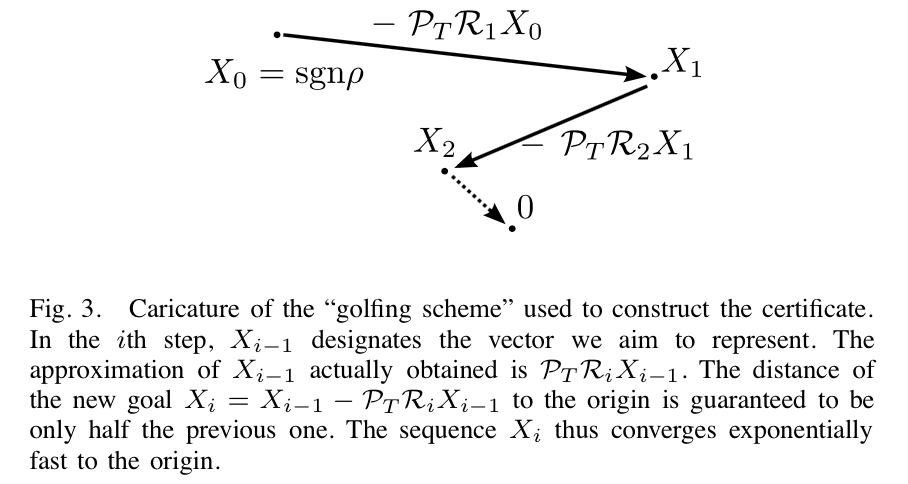
\includegraphics[width=9cm]{3.png}
\label{fig:3}
\end{figure}

We will call this adapted strategy the {\color{red}\textit{golfing scheme}}.

Size $k$: on the one hand, $k$ have to be large enough to allow for the application of the operator large-deviation bounds tailored for \textit{independent} random variables. On the other hand, $k$ must not be too large, as the speed of convergence is ecponential in $l = m/k$.

\subsubsection{Proof:}Before supplying the details of this scheme, we state a lemma which will allow us to control the operator norm $\|\mathcal{P}_T^\perp Y\|_{op}$ of the approximations. The operator-Bernstein inequality makes this a simple calculation.
\textbf{Lemma 7.} \textit{Let $F\in T$. Then}
\[
\mathbb{P}\left[ \| \mathcal{P}_T^\perp \mathcal{R}F\|_{op} > t\right] \le 2n \exp \left( -\dfrac{t^2\kappa r}{4\nu \|F\|_F^2}\right)
\]
for $t \le \sqrt{2/r}\|F\|_F$ and,
\[
\mathbb{P}\left[ \| \mathcal{P}_T^\perp \mathcal{R}F\|_{op} > t\right] \le 2n \exp \left( -\dfrac{t\kappa \sqrt{r}}{2\sqrt{2}\nu \|F\|_F}\right)
\]
for large values of $t$.

\begin{proof}
It is sufficient to treat the case where $\|F\|_F=1$. Set
\[
X_a = \dfrac{n^2}{m}\mathcal{P}_T^\perp w_a(w_a,F).
\]
Then $\sum_i^m X_{A_i} = \dfrac{1}{m}\mathcal{P}_T^\perp F$, and
\[
\mathbb{E}[X_{A_i}] =  \dfrac{1}{m}\mathcal{P}_T^\perp F=0.
\]
Using the property of incoherence $\underset{a} {\mathrm{max}} ~\|w_a\|_{op}^2 \le \nu \dfrac{1}{n}$ and the fact that $\|\mathcal{P}_T^\perp w_a\|_{op} \le \|w_a\|_{op}$ we estimate the variance:
\begin{equation}
\begin{aligned}
\|\mathbb{E}[X_{A_i}^2]\|_{op} &=\|\mathbb{E}[\dfrac{n^4}{m^2}\mathcal{P}_T^\perp w_a(w_a,F)\mathcal{P}_T^\perp w_a(w_a,F)]\|_{op}\qquad \text{(expectation of discrete r.v.)}\\
& = \frac{n^4}{m^2}\|\frac{1}{n^2}\sum_a(w_a,F)^2(\mathcal{P}_T^\perp w_a)^2\|_{op}\\
& \le \dfrac{n^2}{m^2}\sum_a(w_a,F)^2\|(\mathcal{P}_T^\perp w_a)^2\|_{op} \\
& \le \dfrac{n^2}{m^2}\dfrac{\nu}{n}\|F\|_F^2 = \dfrac{n\nu}{m^2} = \dfrac{\nu}{m\kappa r} := V_0^2
\end{aligned}
\label{eq:37}
\end{equation}
Next,
\begin{equation}
\begin{aligned}
\|X_{A_i}\|_{op} &= \frac{n^2}{m}\|\mathcal{P}_T^\perp w_{A_i}(w_{A_i},F)\|_{op}\\
&=\frac{n^2}{m}(\mathcal{P}_T w_{A_i},F)\|\mathcal{P}_T^\perp w_{A_i}\|_{op} \quad (\text{since }F\in T)\\
&\le\frac{n^2}{m}(\mathcal{P}_T w_{A_i},F)\|w_{A_i}\|_{op} \quad (\text{since }\mathcal{P}_T^\perp w_{A_i} \le w_{A_i})\\
&=\frac{n^2}{m}\|\mathcal{P}_T w_{A_i}\|_F\|F\|_F\|w_{A_i}\|_{op}\\
&= \frac{n^2}{m}\sqrt{\frac{2\nu r}{n}\cdot 1\cdot \frac{\nu}{n}}\\
&=\frac{n\nu \sqrt{2r}}{m} \\
&= \frac{\sqrt{2}\nu}{\sqrt{r}\kappa},
\end{aligned}
\end{equation}

so that
\[
\frac{2mV_0^2}{\|X_{A_i}\|_{op}}\ge \frac{2m\nu}{m\kappa r}\frac{\sqrt{r} \kappa}{\sqrt{2}\nu} = \frac{\sqrt{2}}{\sqrt{r}}
\]
Now use Theorem 6.
\end{proof}

We sample $l$ batches of basis elements, the $i$th set consisting of $m_i=\kappa_i rn$ matrices.

For $1\le i \le l$, let
\[
\mathcal{R}: \sigma \mapsto \frac{n^2}{m_i}\sum_{j=m_1+\dots+m_{i-1}+1}^{m_1+\dots+m_i} w_{A_i}( w_{A_i},\sigma)
\]
be the $i$th sampling operator associated with the $i$th batch and set
\[
X_0 = \text{sgn}\rho, \qquad Y_i = \sum_{j=1}^i\mathcal{R}_j X_{j-1}, \qquad X_i = \text{sgn}\rho - \mathcal{P}_TY_i
\]
From this, we get
\begin{equation}
X_i = (\mathbb{1}-\mathcal{P}_T\mathcal{R}_j\mathcal{P}_T)(\mathbb{1}-\mathcal{P}_T\mathcal{R}_{j-1}\mathcal{P}_T)\dots(\mathbb{1}-\mathcal{P}_T\mathcal{R}_1\mathcal{P}_T)X_0
\end{equation}
Assume the in the $i$th run
\begin{equation}
\| (\mathbb{1}-\mathcal{P}_T\mathcal{R}_i\mathcal{P}_T) X_{i-1}\|_F < c_i\|X_{i-1}\|_F
\label{eq:39}
\end{equation}
Denote $p_{op}(i)$ be the probability of this event not occurring. Clearly, if (\ref{eq:39}) does hold for all $i$, then
\[
\|X_i\|_F = \|(\mathbb{1}-\mathcal{P}_T\mathcal{R}_i\mathcal{P}_T) X_{i-1}\|_F \le c_i\|X_{i-1}\|_F
\]
So that $\|X_A{_i}\|_F \le \sqrt{r}\prod_{j=1}^i c_j$.

Assume further that for all $i$ the estimate 
\[
\|\mathcal{P}_T^\perp \mathcal{R}_i X_{i-1}\|_{op} \le t_i\|X_{i-1}\|_F
\] 
is true, with $p_3{i}$ bounding the probability of failure.
Then
\[
\|\mathcal{P}_T^\perp Y_l\|_{op} \le \sum_{i=1}^l\|\mathcal{P}_T^\perp \mathcal{R}_j X_{j-1}\|_{op} \le \sum_{i=1}^l t_i \|X_{i-1}\|_F.
\]

A first simple choice of parameters (to ne refined in section \uppercase\expandafter{\romannumeral2} is
\begin{align*}
& c_i\quad =\quad 1/2\\
& t_i\quad =\quad 1/(4/\sqrt{r})\\
& \kappa_i\quad = \quad 64\nu(\ln(4nr)+\ln(2l)+\beta \ln n)
\end{align*}
for some $\beta > 0$. It follows that 
\[
\|X_i\|_F \le \sqrt{r}2^{-i}, \qquad \|\mathcal{P}_T^\perp Y_l\|_{op} \le \frac{1}{4} \sum_{i=1}^l 2^{-(i-1)} < \frac{1}{2}
\]
with $l = [\log_2(2n^2\sqrt{r})]$, the conditions in Equation (\ref{eq:35}) are met. Using Lemma 5 and Lemma 7 te failure probabiliries become
\begin{align*}
&p_1 \qquad \le \quad 4nr \exp \left( -\frac{\kappa}{32\nu}\right),\\
&p_{op}(i)\quad \le \quad  4nr \exp \left( -\frac{\kappa_i}{32\nu}\right),\\
&p_3(i)\quad \le \quad  2nr \exp \left( -\frac{\kappa_i}{64\nu}\right)
\end{align*}
all of which are bounded above by $\frac{1}{2l}n^{-\beta}$. Theorem 3 for Fourier-type bases thus follows from a simple application of the union bound. The number of coefficients sampled must exceed
\begin{align*}
m &=l\kappa_i = 64\nu(\ln(4nr)+\ln(2l)+\beta \ln n)\log_2(2n^2\sqrt{r})rn\\
& = O(rn\nu (1+\beta)\ln^2n)
\end{align*}


\subsection{\textit{\uppercase\expandafter{\romannumeral5}. The certificate: general case}}

In this section, we show that the construction of $Y$ described above continues to work if the assumption by $\underset{a} {\mathrm{max}} ~\|w_a\|_{op}^2 \le \nu \frac{1}{n}$ on the operator norm of the basis elements is replaced by the incoherence properties 
\begin{align*}
\underset{a} {\mathrm{max}} ~\|\mathcal{P}_Tw_a\|_F^2 &\le 2\nu \frac{r}{n},\\
\underset{a} {\mathrm{max}} ~~(w_a,\text{sgn}\rho)^2 &\le \nu\frac{r}{n^2}
\end{align*}

Indeed, in the discussion of the golfing scheme, we reffered to the operator norm of $w_a$ exactly once. In the proof of Lemma 7, we considered the quantity
\begin{equation}
X_a = \frac{n^2}{m}\mathcal{P}_T^\perp w_a(w_a, F).
\end{equation}
After Equation (\ref{eq:37}), the variance
\[
\|\mathbb{E}[X_{A_i}^2]\|_{op} \le \frac{n^2}{m^2}\sum_a(w_a,F)^2\|(\mathcal{P}_T^\perp w_a)^2\|_{op}
\]
was upper-bounded using the fact that $\|(\mathcal{P}_T^\perp w_a)^2\|_{op} \le \frac{\nu}{n}$. Clearly the absence of this assumption can be compensated for by a suitable bound on $(w_a,F)^2$. This will be made precise below.

Assume that $F$ os sp,e ,atrox om $T$ with $\|F\|_F = 1$. Further, assume that at least one of the following two bounds
\begin{align}
\underset{a} {\mathrm{max}} ~\|w_a\|_{op}^2 & \le \frac{v}{n}\\
\underset{a} {\mathrm{max}} ~|(w_a,F)|^2 & \le \frac{v}{n^2}
\end{align}
holds.

Note that
\begin{equation}
\|\mathbb{E}[X_{A_i}^2]\|_{op} \le \frac{n^3}{m^2}underset{\psi} {\mathrm{max}} ~\sum_a(w_a,F)^2\frac{1}{n}<\psi,w_a^2\psi>,
\label{eq:43}
\end{equation}
where the maximum is over all normalized vectors $\psi \in (range  \, \rho)^\perp$. Let $\psi_0$ be a vector achieving the maximum. Define two vectors $p,q$ in $\mathbb{R}^{n^2}$ by setting their components to 
\begin{equation}
q_a := (w_a,F)^2, \qquad p_a := \frac{1}{n}<\psi_0,w_a^2\psi_0>
\label{eq:44}
\end{equation}

The assumption that $\|F\|_F^2 = 1$ implies that $\|q\|_1 = \sum_a|q_a| = 1$. Slightly less obvious is the fact thatthe same is true for the other vector. $\|p\|_1 = 1$, regardless of the basis chosen. This relation is ascertained by the next lemma.

\textbf{Lemma 8}. \textit{Let $\lbrace w_a \rbrace$, be a set of $n \times n-matrices$ (not necessarily Hermitian) that fulfill the completness relation}
\begin{equation}
\sum_a(\bar{w}_a)_{i_1,j_1}(w_a)_{i_{op},j_{op}} = \delta_{i_1,i_{op}}\delta_{i_{op},j_{op}}.
\end{equation}
\textit{Then}
\[
\sum_a w_a^* w_a = n\mathbb{1}
\]

\begin{proof}
Compute:
\[
\left(\sum_a w_a^* w_a\right)_{i,j} = \sum_{a,k}(\bar{w}_a)_{k,i}(w_a)_{k,j} = \sum_k \delta_{i,j} = n\delta_{i,j}
\]
\end{proof}

Thus,
\[
\|p\|_1 = \sum_ap_a = \frac{1}{n}<\psi_0,n\mathbb{1}\psi_0>
\]

We return to the vectors in (\ref{eq:44}). The assumptions made imply that at least one of the vectors is element-wise bounded above by $\frac{\nu}{n^2}$.Thus
\begin{equation}
\left|\sum_ap_aq_a\right| \le \min\lbrace \|p\|_1 \|q\|_\infty,\|p\|_\infty \|q\|_1 \rbrace \le \frac{\nu}{n^2}
\end{equation}
Plugging this estimate into the computation of the variance (\ref{eq:43}) we obtin
\[
\mathbb{E}[X_{A_i}^2]\|_{op} \le \frac{n^3}{m^2}\frac{\nu}{n^2} = \frac{\nu}{m\kappa r}.
\]
We have proved the general analogue of Lemma 7:

\textbf{Lemma 9.} \textit{Let $F \in T$. Let $f\ge \|F\|_F$ be an upper bound on the Frobenius norm of F. Assume that one of the two bounds}
\begin{align}
\underset{a} {\mathrm{max}} ~\|w_a\|_{op}^2 & \le \frac{v}{n}\\
\underset{a} {\mathrm{max}} ~|(w_a,F)|^2 & \le \frac{v}{n^2}f^2
\end{align}
\textit{holds}. \textit{Then}

\begin{equation}
\mathbb{P} \left[  \|\mathcal{P}_T^\perp\mathcal{R}F\|_{op} >t    \right] \le 2n \exp\left(-\frac{t^2\kappa r}{4\nu f^2} \right),
\end{equation}
\textit{for $t\le \sqrt{2/r}f$.}

Next, we have to justify the bounds on $(w_a,F)^2$ we imposed in the previous lemma, By assumption $\underset{a} {\mathrm{max}} ~(w_a,\text{sgn}\rho)^2 \le \nu\frac{r}{n^2}$, the estimate does hold for $F = \text{sgn} \rho$, i.e. Lemma 9 may be applied during the first leg $X_0 = \text{sgn} \rho$ of the ``golfing scheme''. However, there is no a priori reason that the same be true for $X_1 = (\mathbb{1}-\mathcal{P}_T\mathcal{R}_1\mathcal{P}_T)X_0$. For nor, all we know about $X_1$ is that it is an element of T and hence low-rank. This property was enough for Fourier-type bases, but in the general case, it proves too weak. We thus hae to ensure that``inhomogeneity'' of $X_i$ implies inhomoheneity of $X_{i+1}$, a fact that can be ascertained using yet another Chernoff bound.

Let $\mu(F) = \underset{a} {\mathrm{max}} ~(w_a,F)^2$ be the maximal squared overlap between $F$ and any element of the operator basis.

\textbf{Lemma 10.}\textit{Let $F \in T$. Then}
\[
\mathbb{P}[ \mu(\mathbb{1}-\mathcal{P}_T\mathcal{R}\mathcal{P}_T)F > t] \le 2n^2 \exp \left( -\frac{t\kappa}{4\mu(F)\nu}\right)
\]
\textit{for all $t \le \mu(F)$}.
\begin{proof}
Fix $b \in [1,n^2]$. Define
\begin{equation}
X_a = \frac{1}{m}(w_a,F)-(w_b,\frac{n^2}{m}\mathcal{P}_Tw_a)(w_a,F).
\label{eq:50}
\end{equation}  

Then
\[
\sum_i^m X_{A_i} = (w_b,(\mathbb{1}-\mathcal{P}_T\mathcal{R}\mathcal{P}_T)F).
\]
Note that the first term in (\ref{eq:50}) is the expectation value of the second one. Therefore, $\mathbb{E}[X_{A_i}]=0$ and the variance of $X_{A_i}$ is bounded above by the variance of the second term alone (as in the proof of Lemma 5):
\begin{align*}
\mathbb{E}[X_{A_i}^2] & \le \frac{1}{n^2}\sum_a(w_b,\frac{n^2}{m}\mathcal{P}_Tw_a)^2(w_a,F)^2\\
& \le \frac{n^2}{m}\mu(F)\sum_a(\mathcal{P}_Tw_b,w_a)^2\\
& =  \frac{n^2}{m}\mu(F)\|\mathcal{P}_Tw_b\|_F^2\\
& \le \frac{n^2\mu(F)\nu r}{m^2n}\\
& = \frac{\mu(F)\nu}{m\kappa} =: V_0^2
\end{align*}
Further,
\[
|X_{A_i}| \le \frac{1}{m}\mu(F)^{1/2}\left(1+n^2\frac{\nu r}{n}\right) = \frac{1}{m}\mu(F)^{1/2}(1+n\nu)r.
\]
Thus, from the Chernoff bound:
\begin{align*}
& \mathbb{P}\left[|(w_b,(\mathbb{1}-\mathcal{P}_T\mathcal{R}\mathcal{P}_T)F))|> \sqrt{t} \right] 
&\le 2\exp\left(-\frac{t\kappa}{4\mu(F)\nu}\right)
\end{align*}
as long as $\sqrt{t}$ does not exceed
\[
\frac{2mV_0^2}{|X_{A_i}|} = \frac{2m\mu(F)\nu}{m\kappa}\frac{m}{\mu(F)^{1/2}(1+n\mu r)}\le \mu(F)^{1/2}
\]

The advertised estimate follows by taking squares and applying the union bound over the $n^2$ elements of the basis.
\end{proof}

With these preparations made, we can repeat the ``golfing'' argument from the last section. As an additional constraint, we demand that
\[
\mu(X_i) \le c_i^2\mu(X_{i-1})
\]
be fulfilled for all $i$, with probabiliry of failure given by $p_4(i)$.

Then, with
\begin{align*}
& c_i\quad =\quad 1/2\\
& t_i\quad =\quad 1/(2/\sqrt{r})\\
& \kappa_i\quad = \quad 64\nu(\ln(4n^2)+\ln(3l)+\beta \ln n)
\end{align*}
it follows that
\[
\|X_i\|_F \le 2^{-i}\|\text{sgn} \rho\|_F = 2^{-i}\sqrt{r},\\
\mu(X_i) \le 2^{-2i}\mu(\text{sgn} \rho) \le \frac{\nu}{n^2}(2^{-2i}r).
\]
Thus, in $i$th iteration of the golfing scheme, we can apply Lemma 9 with $F = X_i$ and $f = 2^{-i}\sqrt{r}$.

The failure probabilities $p_1,p_{op}(i),p_3(i)$ are as before. Further
\[
p_4(i) \le 2n^2 \exp\left( -\frac{\kappa_i}{16\nu} \right),
\]
which, as the other probabilities, is bounded above by $\frac{1}{3l}n^{-\beta}$. By the union bound, Theorem 3 holds as long as 
\[
m > \log_2(2n^2\sqrt{r}) 64\nu(\ln(4n^2)+\ln(3l)+\beta\ln n) rn
\]

\end{document}